\documentclass[10pt]{article}
\usepackage[polish]{babel}
\usepackage[utf8]{inputenc}
\usepackage[T1]{fontenc}
\usepackage{graphicx}
\usepackage[export]{adjustbox}
\graphicspath{ {./images/} }
\usepackage{amsmath}
\usepackage{amsfonts}
\usepackage{amssymb}
\usepackage[version=4]{mhchem}
\usepackage{stmaryrd}

\title{Zestaw 7 }

\author{}
\date{}


\begin{document}
\maketitle
\begin{center}

\includegraphics[max width=\textwidth]{2024_11_21_e31b2faaa846039f7212g-1}
\end{center}

\section*{GIMNAZJUM}
\begin{enumerate}
  \item W trójkącie prostokątnym suma długości przyprostokątnych wynosi \(\sqrt{18}\), a przeciwprostokątna ma długość 4. Oblicz pole tego trójkąta.
  \item Wykaż, że krawędzi sześcianu nie można ponumerować liczbami od 1 do 12 tak, by suma numerów krawędzi wychodzących z każdego wierzchołka była taka sama. Czy można spełnić ten warunek numerując krawędzie dwunastoma różnymi liczbami ze zbioru \{1, 2, 3, ..., 13\}?
  \item Oblicz pole pięciokąta wypukłego \(A B C D E\), w którym boki \(A B, C D\) i \(E A\) mają długość 1, a suma długości boków \(B C\) i \(D E\) wynosi 1 oraz kąty \(A B C\) i \(D E A\) są proste
\end{enumerate}

\section*{LICEUM}
\begin{enumerate}
  \item Udowodnij, że istnieje nieskończenie wiele par liczb naturalnych ( \(a, b\) ), dla których liczba \(4^{a}+4^{b}+4^{a+b}\)\\
jest kwadratem liczby całkowitej.
  \item Punkty \(E\) i \(F\) leżą odpowiednio na bokach \(B C\) i \(C D\) prostokąta \(A B C D\), przy czym trójkąt \(A E F\) jest równoboczny. Wykaż, że suma pól trójkątów \(A B E\) i \(A D F\) jest równa polu trójkąta \(C E F\).\\
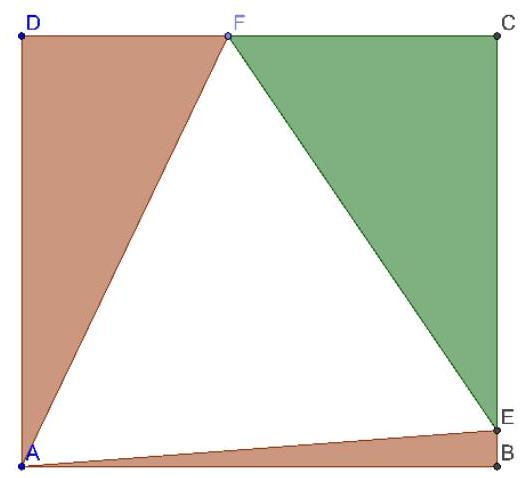
\includegraphics[max width=\textwidth, center]{2024_11_21_e31b2faaa846039f7212g-1(1)}
  \item W czworościanie \(A B C D\) poprowadzono płaszczyznę przechodzącą przez środki krawędzi \(A B, B D\) i \(C D\). Wykaż, że płaszczyzna ta dzieli czworościan na dwie bryły o równych objętościach.
\end{enumerate}

Rozwiązania należy oddać do piątku 13 lutego do godziny 12.30 koordynatorowi konkursu panu Jarostawowi Szczepaniakowi lub swojemu nauczycielowi matematyki.

Na stronie internetowej szkoły w zakładce Konkursy i olimpiady można znaleźć wyniki dotychczasowych rund i rozwiązania zadań.


\end{document}